\documentclass[12pt]{article}

\usepackage{amsmath}
\usepackage{amssymb}
\usepackage{calc}
\usepackage{units}
\usepackage{graphicx}
\usepackage[pdftex]{hyperref}
\usepackage{subfig}
\usepackage[margin=1in]{geometry}
\usepackage{listings}
\usepackage[numbers,sort&compress]{natbib}
\usepackage{bm}
\usepackage{paralist}
\usepackage[draft]{fixme}
\usepackage{textcomp}
\usepackage{yorkdefs}

\newcommand{\halflife}{\ensuremath{T_{\nicefrac{1}{2}}}\xspace}

\hypersetup{
  breaklinks=true,
  pdftitle={Alternating Current RL Circuits},
  pdfauthor={Kevin R. Lynch based on a lab by D.C.Jain}, 
  pdfsubject={Phyiscs, Electricity and magnetism},
  pdfkeywords={resistance, inductance, alternating current},
  pdflang={en-US},
}

\title{Alternating Current RL Circuits}
\author{}
%Kevin R. Lynch, based on an earlier lab by D.C.Jain
%\date{2012-03-16}
\date{}

\begin{document}

\maketitle

\section{Objectives}
\label{sec:objectives}

\begin{enumerate}
\item To understand the voltage/current phase behavior of RL circuits
  under applied alternating current voltages, and
\item To understand the current amplitude behavior of RL circuits
  under applied alternating current voltages.
\end{enumerate}

\section{Introduction}
\label{sec:introduction}

You have studied the behavior of RC circuits under both direct and
alternating current conditions.  The final passive component we need
to consider is the \textit{inductor}.  The voltage across a capacitor
is proportional to the charge on it ($V(t) = q(t)/C$), and the voltage
across a resistor is proportional to the rate at which charge flows
through it ($V_R(t) = R \dd q(t)/\dd t$), while the voltage across the
inductor is proportional to the rate of change of the current
\begin{gather*}
  V_L(t) = - L \deriv{I(t)}{t} = -L \deriv[2]{q(t)}{t}\ .
\end{gather*}
The minus sign indicates that the voltage across the inductor seeks to
minimize the or negate the changing current.

\begin{figure}
  \centering
%  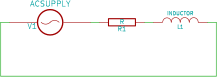
\includegraphics[width=2\textwidth/3]{figures/rl-circuit}
  \caption{The RL circuit.}
  \label{fig:rlcircuit}
\end{figure}
In a previous lab\footnote{\textit{Alternating Current RC Circuits}}
you studied the behavior of the RC circuit under alternating applied
(or AC) voltages.  Here, you will study the behavior of a similar
circuit where the capacitor is replaced with an \textit{inductor}; see
Figure~\ref{fig:rlcircuit}. 

\section{Theory}
\label{sec:theory}

\begin{figure}
  \centering
  \includegraphics[width=2\textwidth/3]{figures/phase}
  \caption{A schematic of the phase difference between the applied
    voltage $V(t)$ and the derived current $I(t)$.}
  \label{fig:phase}
\end{figure}
Once again, let's analyze this circuit using Kirchoff's Rules.  As
always, you find
\begin{gather*}
  V_s(t) - V_R(t) - V_L(t) = 0\ ,
\end{gather*}
leading to the differential equation
\begin{gather*}
  \deriv{I(t)}{t} + \frac{R}{L} I(t) = \frac{V_s(t)}{L}\ .
\end{gather*}
This is, in all important ways, \textit{identical} to the behavior of
the charge on a capacitor.  The time constant for current changes is
here $\tau = L/R$.  Again, we solve the equation in all its
particulars in Appendix~\ref{sec:solutions}.  For a sinusoidally
varying source voltage
\begin{gather*}
  V_s(t) = V_s \cos\omega t\ ,
\end{gather*}
we find the current is again out of phase, but this time it
\textit{leads} the voltage (see Figure~\ref{fig:phase}\fixme{check the
  sign on the inductor voltage}
\begin{gather*}
  I(t) = \frac{V_s}{R} \frac{1}{\sqrt{1 + (\omega \tau)^2}}
  \cos(\omega t - \phi)\\
  V_R(t) = V_s \frac{1}{\sqrt{1 + (\omega \tau)^2}}
  \cos(\omega t - \phi)\\
  V_L(t) = V_s \frac{\omega \tau}{\sqrt{1 + (\omega \tau)^2}}
  \sin(\omega t - \phi)\ ,
\end{gather*}
where the phase is given by 
\begin{gather*}
  \tan \phi = \frac{\omega L}{R}\ .
\end{gather*}

Just as for the capacitor circuit, we can define and use the concept
of \textit{impedance} to predict the behavior of the circuit.  The
combination $\omega L$ has units of resistance, and we
define the \textit{inductive reactance} by
\begin{gather*}
  X_L = \omega L\ .
\end{gather*}
The phase is given by
\begin{gather*}
  \tan\phi = \frac{X_L}{R}\ ,
\end{gather*}
while the circuit impedance is given by
\begin{gather*}
  Z^2 = R^2 + X_L^2\ ,
\end{gather*}
which has all the same consequences for the voltage amplitudes as it
did for the $RC$ circuit.

\begin{figure}
  \centering
  \subfloat[][Phases]{
    \includegraphics[width=\textwidth/2-0.1in]{figures/frequency-phase}
  }
  \subfloat[][Voltage Amplitudes]{
    \includegraphics[width=\textwidth/2-0.1in]{figures/frequency-amplitudes}
  }
  \caption{The phase angle as a function of angular frequency is on
    the left, while the voltage amplitudes are displayed on the
    right.  In both cases, the frequency is normalized in units of
    $L/R$.  The phase is normalized to $\pi/2$, while the amplitudes
    are normalized to $V_s$.}
  \label{fig:frequency}
\end{figure}
Just as we did for the RC circuit, we can consider the behavior of
this circuit as a function of frequency.  In the limit that the
frequency goes to zero, the current will be steady state.  Since
steady state means ``no change'', the voltage across the inductor must
vanish, and the phase has to go to zero.  This is what we see in
Figure~\ref{fig:frequency}.  In the other extreme, with very high
frequencies, the current is changing very quickly, so the voltage will
all be visible across the inductor; again, this is what we see in
Figure~\ref{fig:frequency}.  Inductors become transparent at low
frequencies, and opaque at high frequencies, just the opposite of the
capacitor!

\section{Procedures}
\label{sec:procedures}


\appendix

\section{Derivation of Solutions}
\label{sec:solutions}


\newpage

\section*{Pre-Lab Exercises}

Answer these questions as instructed on Blackboard; make sure to
submit them before your lab session!

\begin{enumerate}
\item Foobar
\end{enumerate}

\newpage

\section*{Post-Lab Exercises}

\begin{enumerate}
\item Discuss briefly whether you have met the objectives of the lab
  exercises.
\end{enumerate}

\end{document}

%%% Local Variables: 
%%% mode: latex
%%% TeX-master: t
%%% End: 
